\chapterauthor{Tim Warburton}

\epigraph{Most authors are not competent designers and make typographic errors -- formatting decisions that make the document harder to read.}{Leslie Lamport, \emph{Document Production: Visual or Logical?}. }

\minitoc

%Warm up: try this three minute challenge to replicate some typeset equations with \LaTeX{} \href{http://texnique.xyz}{http://texnique.xyz}.

%\section{Typesetting documents with \LaTeX{}}

\href{https://www-cs-faculty.stanford.edu/~knuth/}{Donald Knuth} created the \TeX{} typesetting system after being disappointed with the quality of the typesetting of a book he published in the 70s. For more on the history of \TeX{} see \href{https://en.wikipedia.org/wiki/TeX}{wiki}. The \TeX{} system excels at giving an author control over every aspect of the appearance of a document down to painstaking  positioning of objects to high precision. However, using the \TeX{} system is more akin to creating a computer program that when compiled results in a document. This means it has quite a steep learning curve. Think: learning a programming language specifically tailored to creating documents.

To help make it easier to typeset a document \href{http://www.lamport.org}{Leslie Lamport} created a higher level macro based language called \href{https://en.wikipedia.org/wiki/LaTeX}{\LaTeX{}}. This is perhaps the most commonly used type setting system  built around \TeX{}. In fact for better or worse these lecture notes have been typeset using \LaTeX{}. 

% custom size
\begin{figure}[htbp!]
    \centering
    \fbox{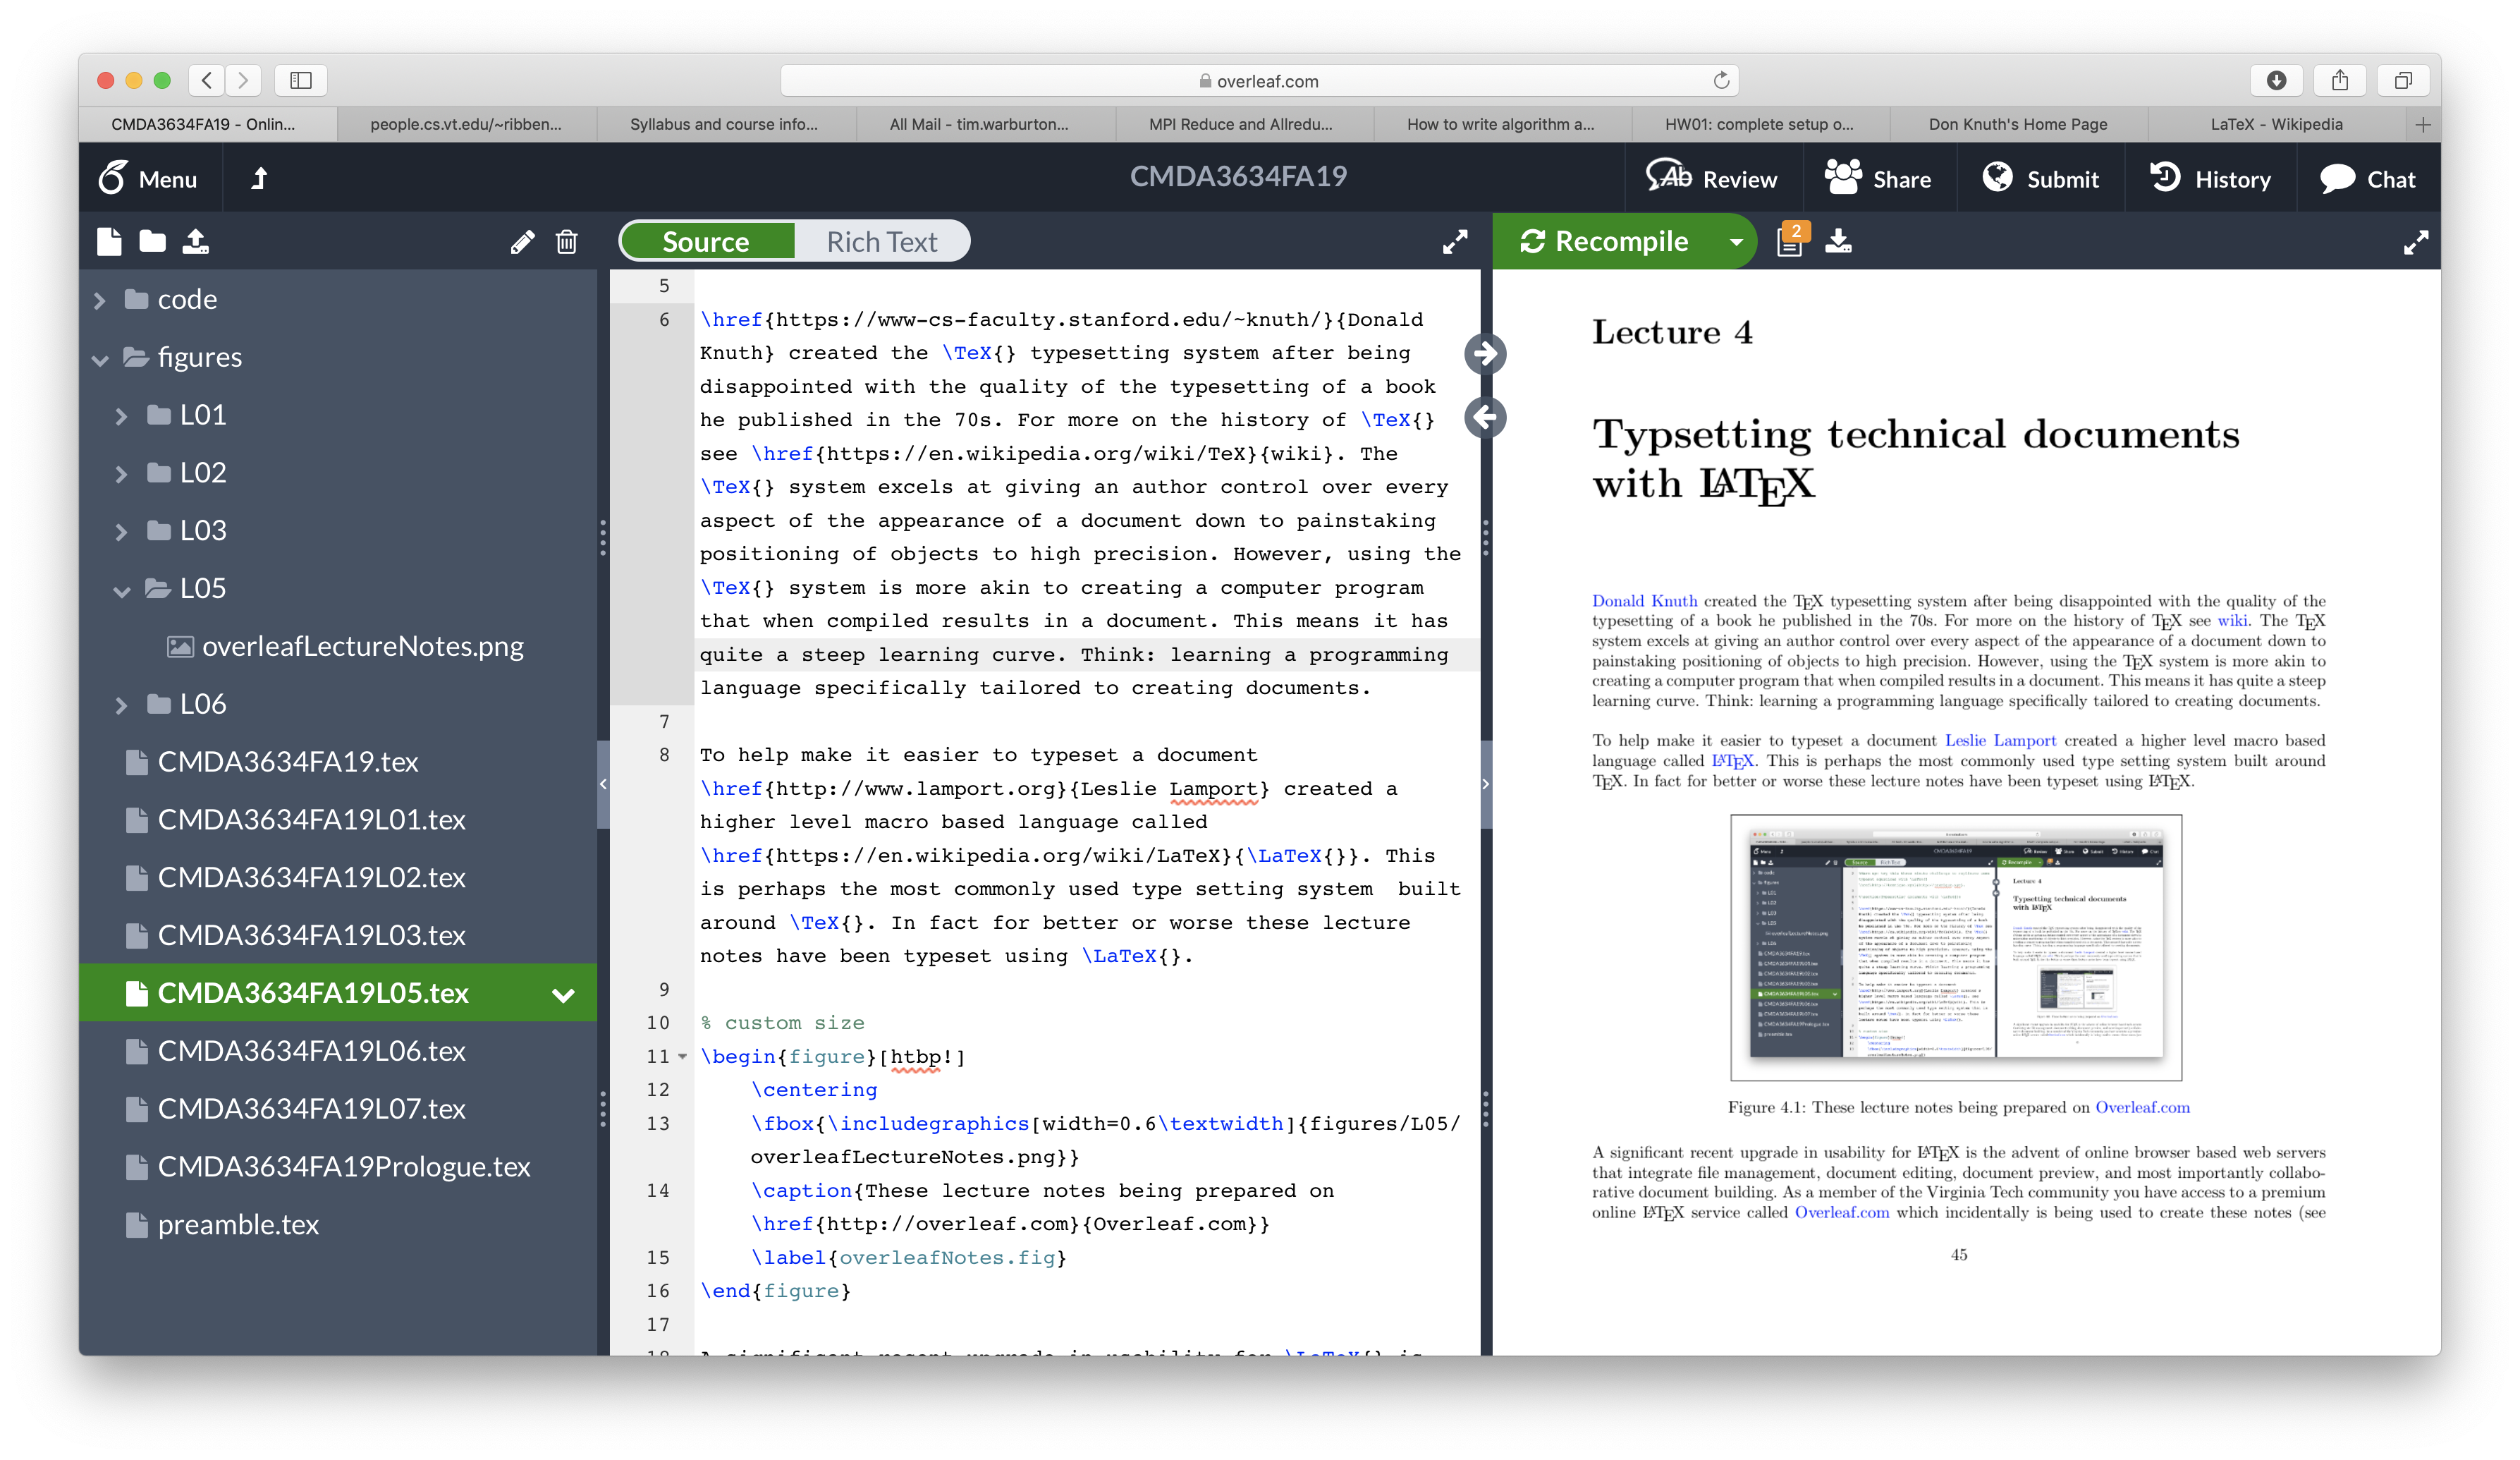
\includegraphics[width=0.6\textwidth]{figures/L05/overleafLectureNotes.png}}
    \caption{These lecture notes being prepared on \href{http://overleaf.com}{Overleaf.com}}
    \label{overleafNotes.fig}
\end{figure}

A significant recent upgrade in usability for \LaTeX{} is the advent of online browser based web servers that integrate file management, document editing, document preview, and most importantly collaborative document building. As a member of the Virginia Tech community you have access to a premium online \LaTeX{} service called  \href{http://overleaf.com}{Overleaf.com} which incidentally is being used to create these notes (see Figure \ref{overleafNotes.fig}.

\section{Getting started with \LaTeX{} on \href{http://overleaf.com}{Overleaf.com}}

For this lecture you should go ahead and create a user account with \href{http://overleaf.com}{Overleaf} if you have not already set an account up.

After you have signed into your new Overleaf account you will land on the projects page. Click on the green ``New Project'' button and select ``Blank Project''. Enter a name for your project, say CMDA3634FA19L01[YOUR LAST NAME], and click on the ``Create'' button. Overleaf will then present you with a prepopulated project as shown in Figure \ref{overleafBlankProject.fig}. 

\begin{figure}[htbp!]
    \centering
    \fbox{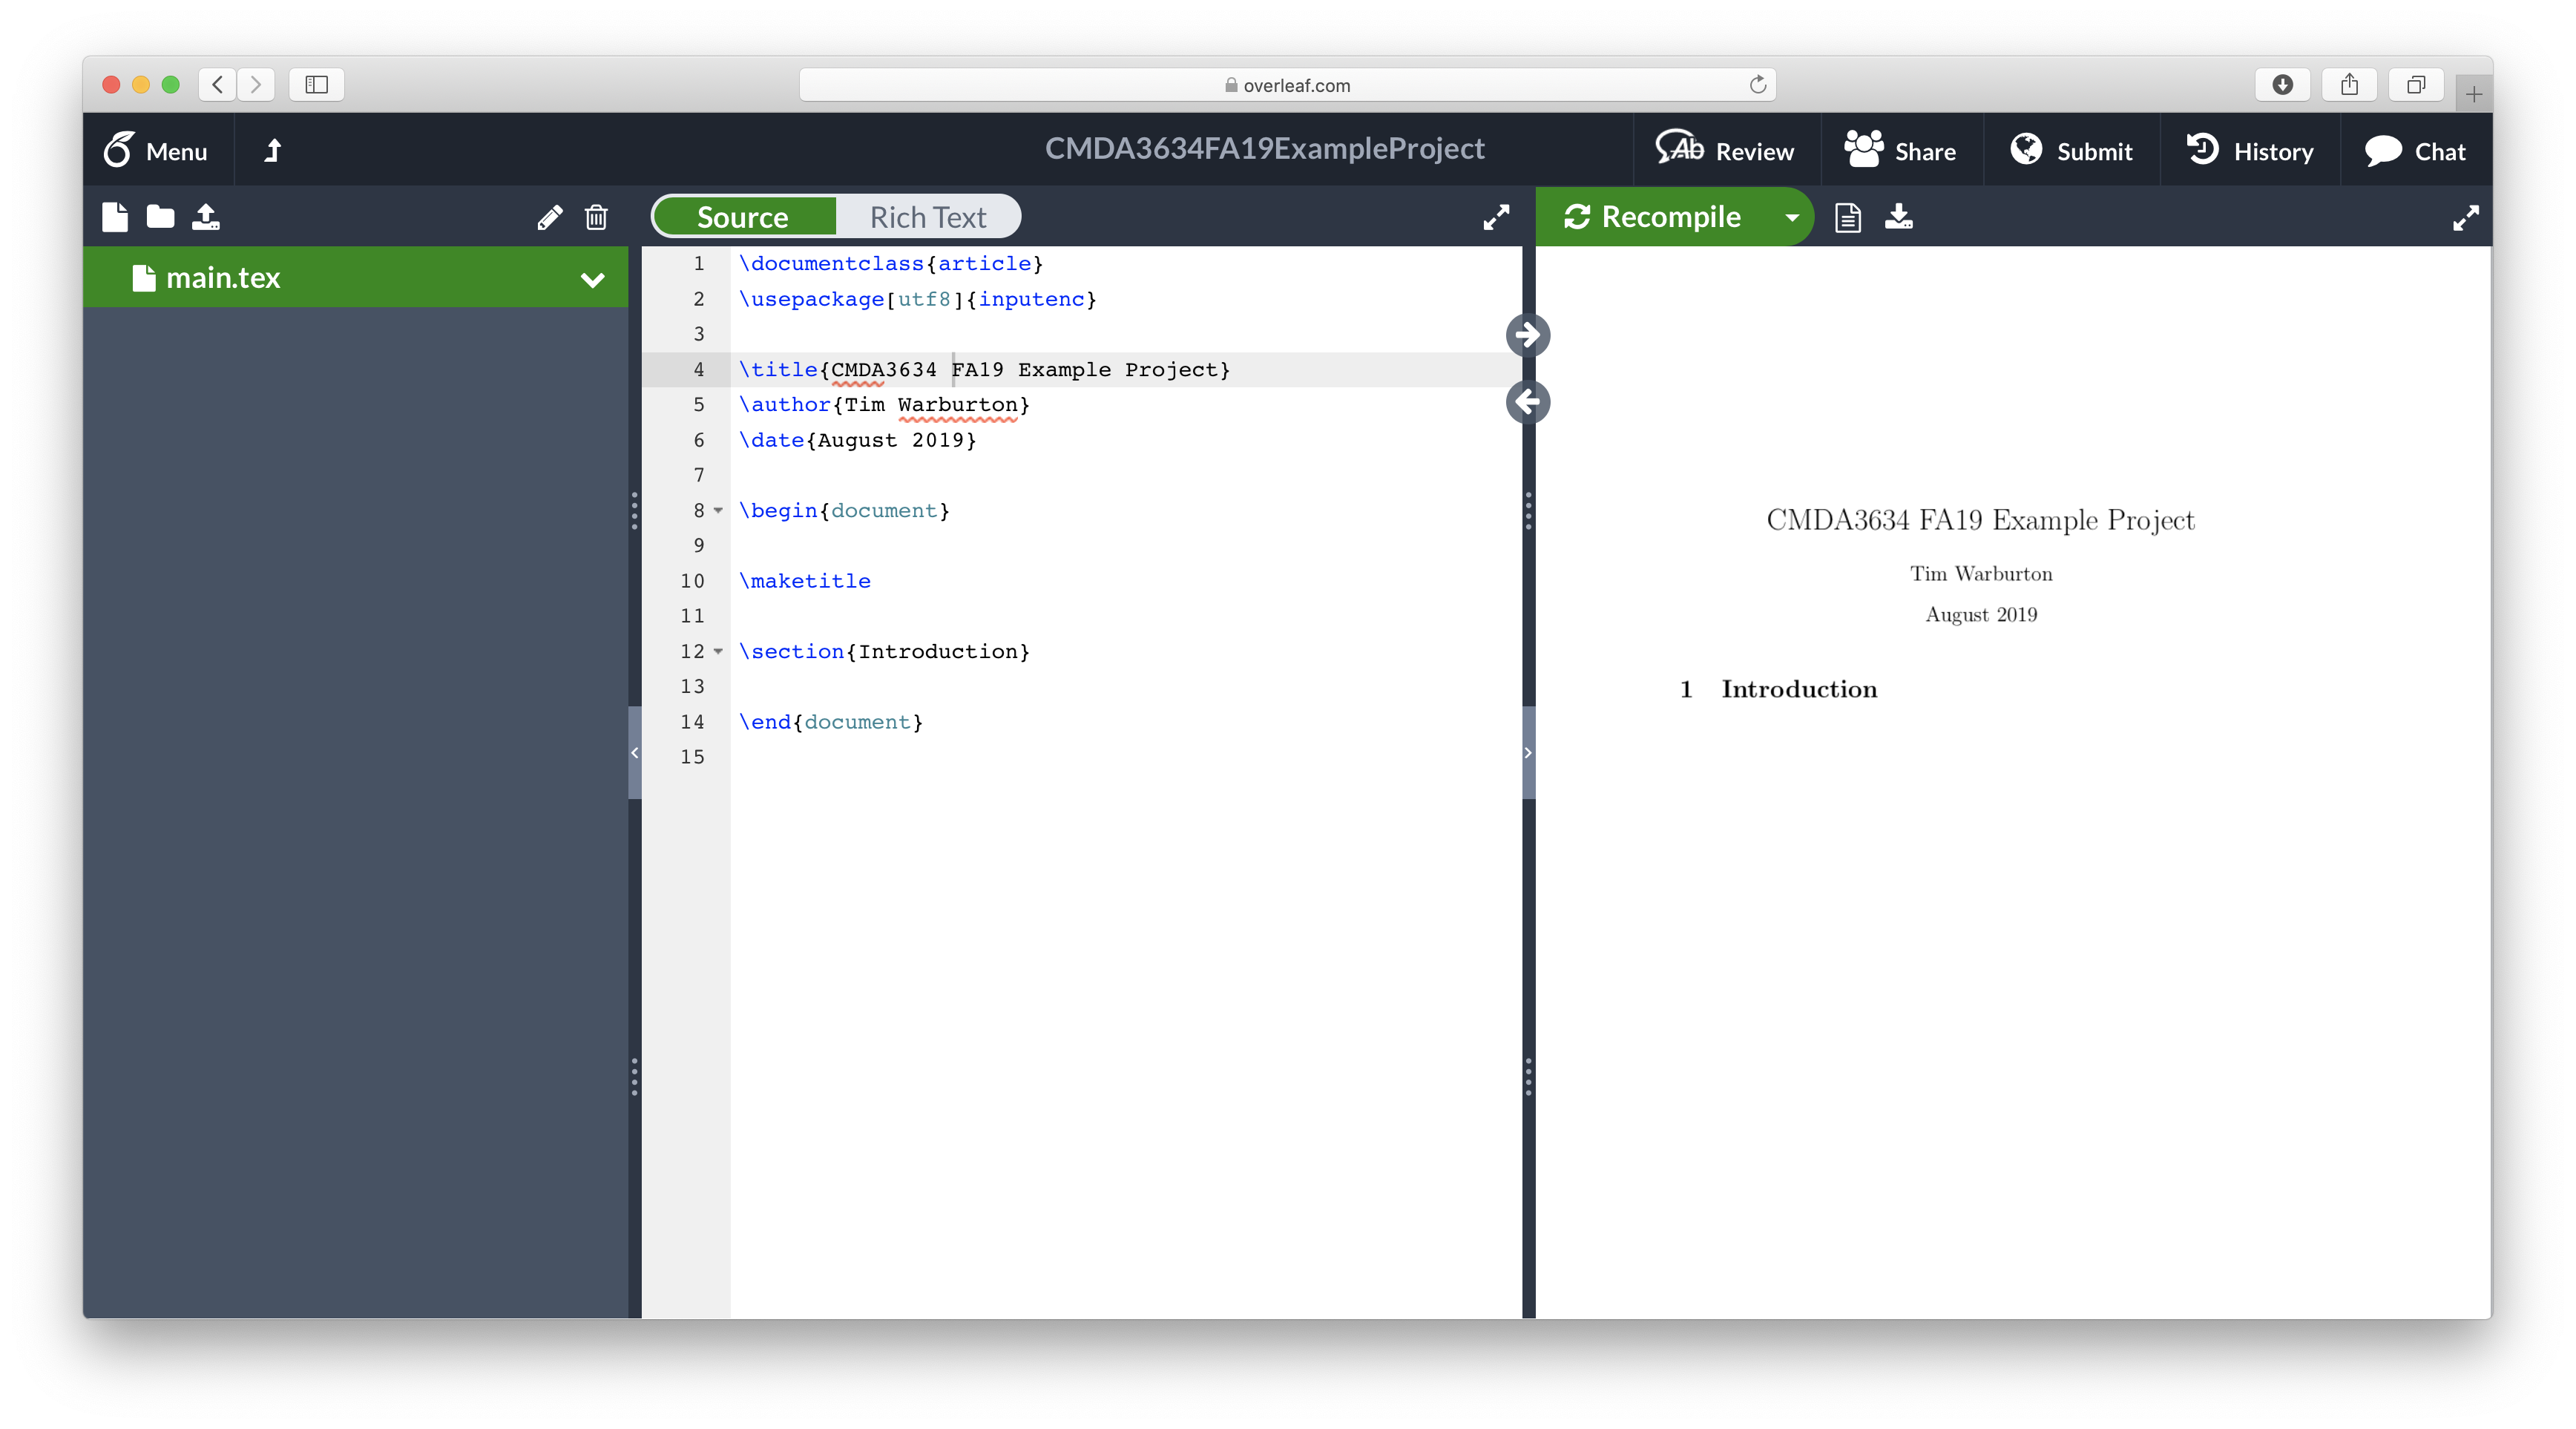
\includegraphics[width=0.98\textwidth]{figures/L05/overleafBlankProject.png}}
    \caption{Blank project created on \href{http://overleaf.com}{Overleaf.com}. Image shows user interface for editing a \LaTeX{} project. Left: project file manager. Middle: text document editor. Right: preview of compiled document. }
    \label{overleafBlankProject.fig}
\end{figure}

There are four important elements in the Overleaf project interface. Clicking the Menu button at the top left will reveal several options for configuring the project. The left pane is the file browser for the project. The middle pane is an editor for the a project text file. On the right is a preview of the compiled project.

\begin{figure}[htbp!]
    \centering
    \fbox{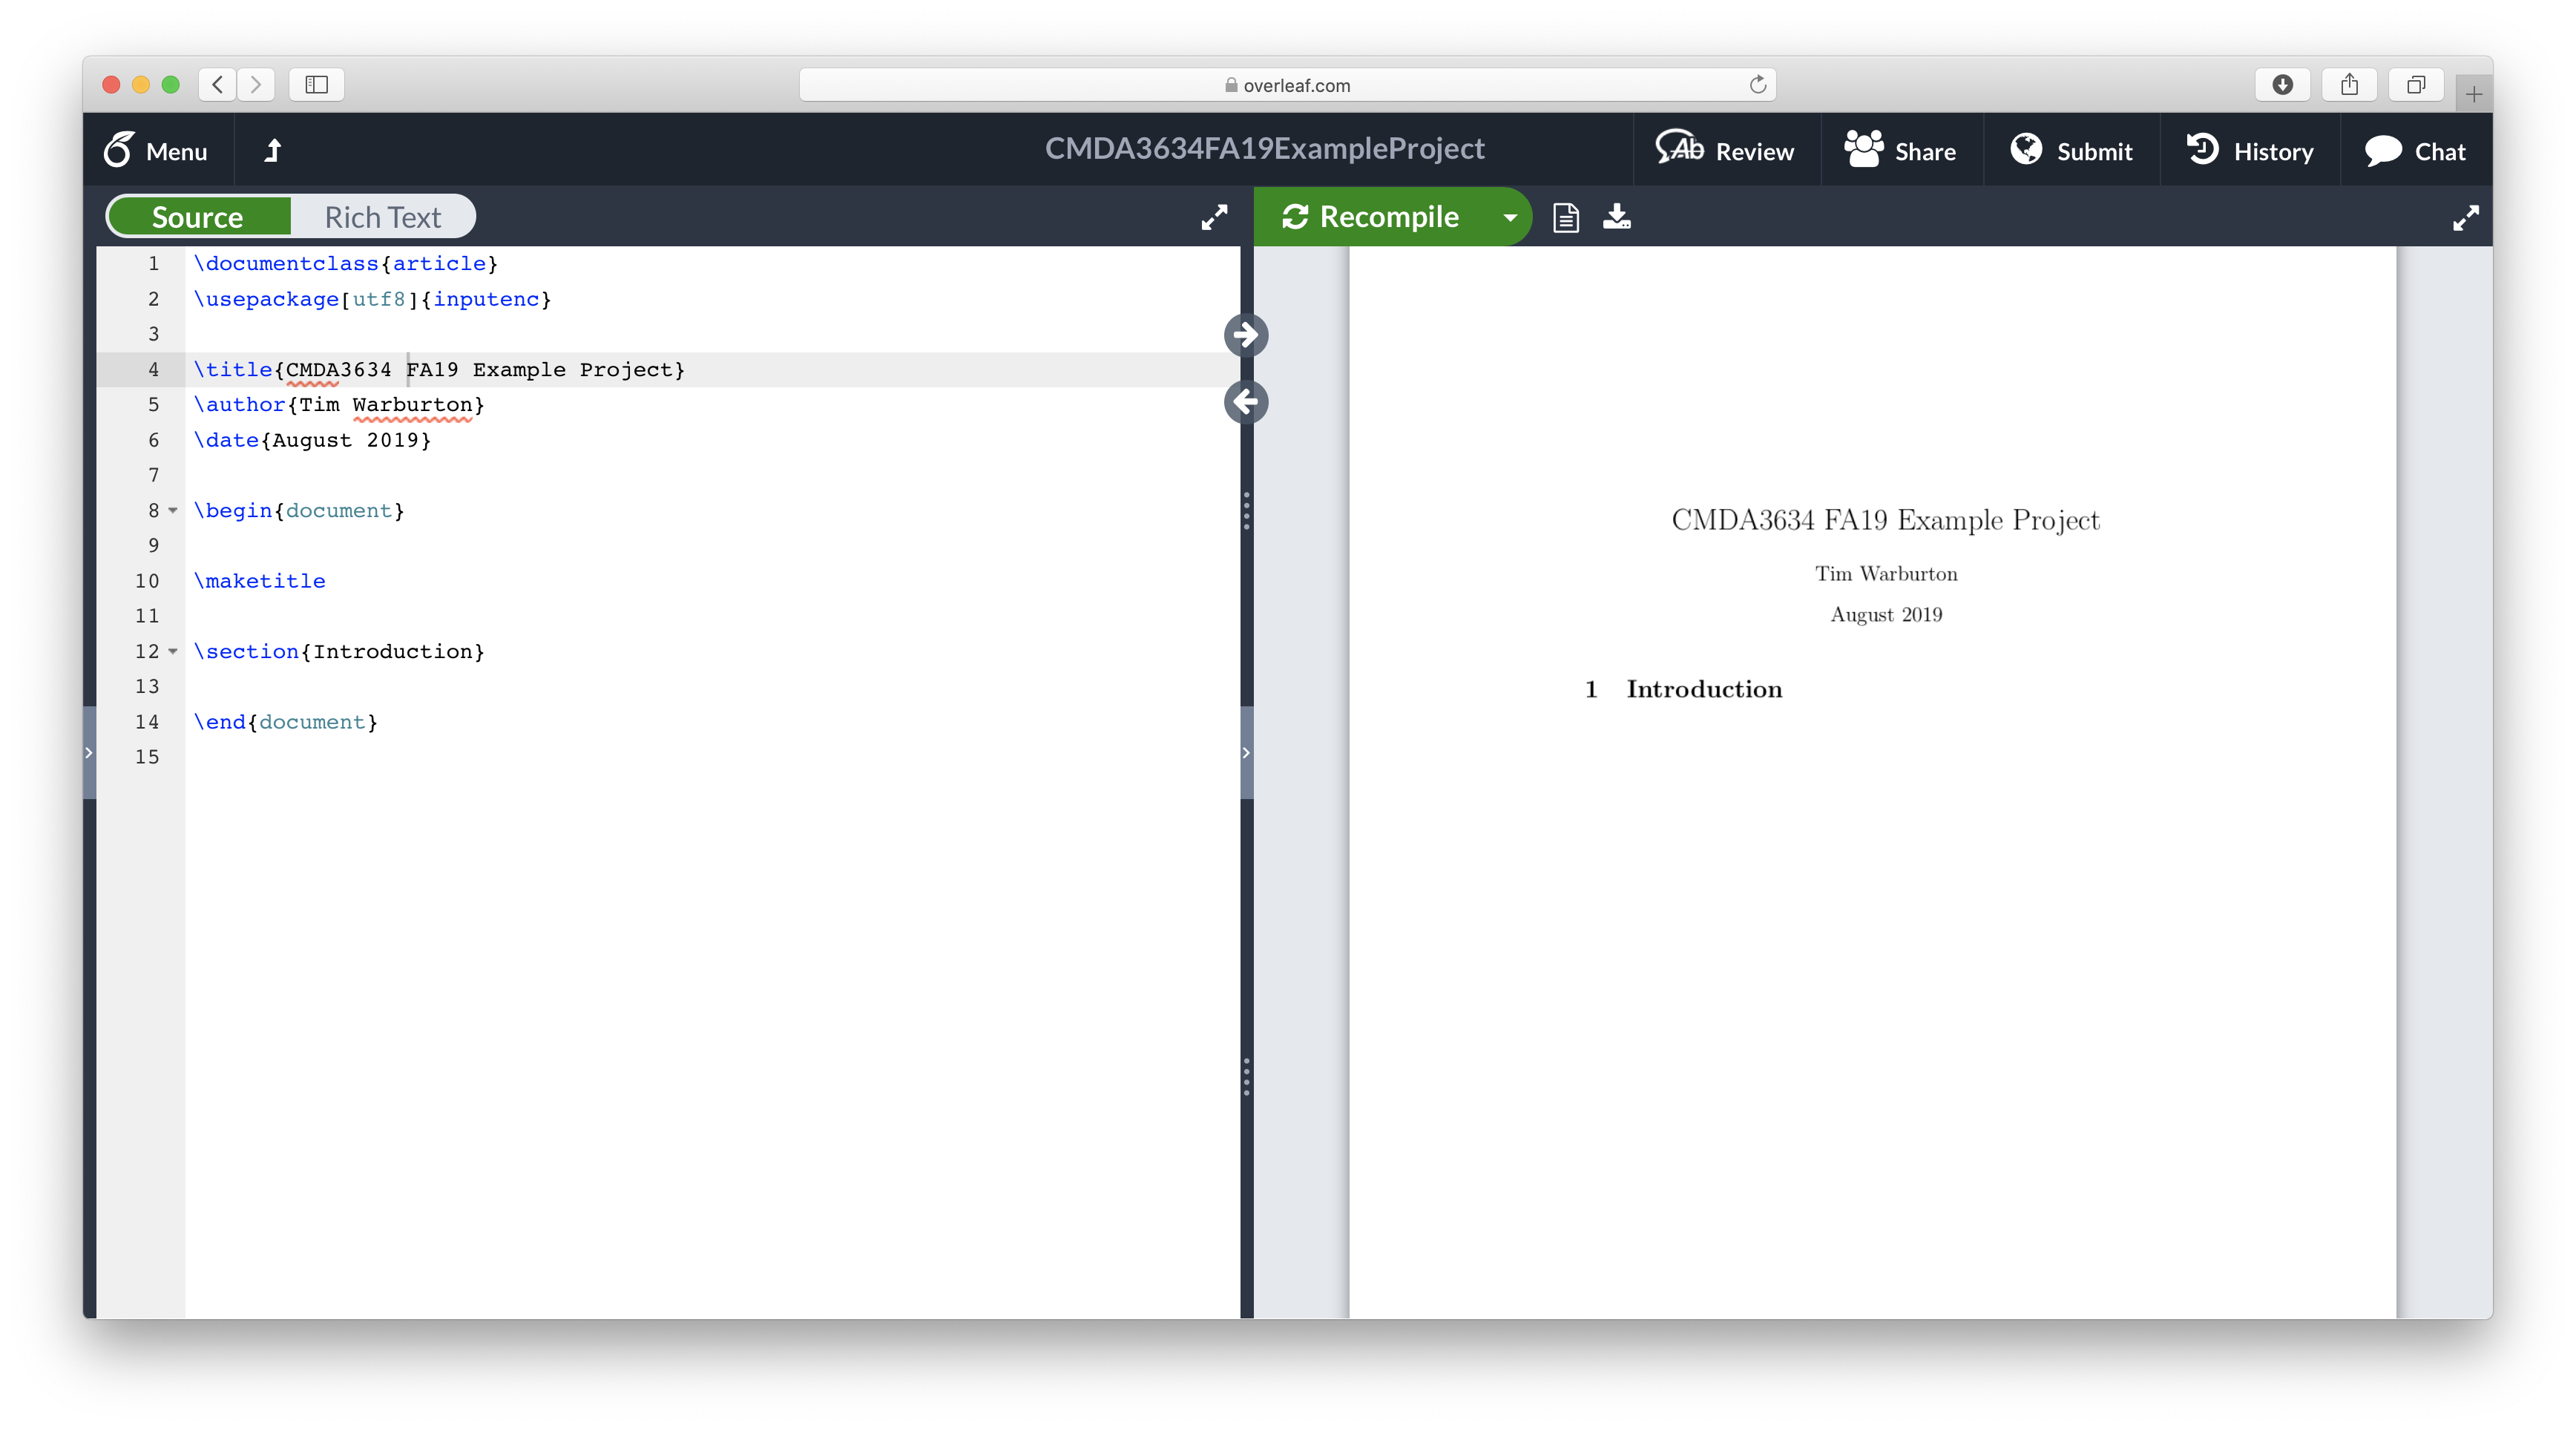
\includegraphics[width=0.98\textwidth]{figures/L05/overleafBlankProjectCollapsedFileBrowser.png}}
    \caption{File browser hidden by clicking on the small arrow to the left of the editor pane.}
    \label{overleafBlankProjectCollapsedFileBrowser.fig}
\end{figure}

\newpage
For simplicity we will only use a single text document for this project and for the time being we can hide the document browser (by clicking the arrow at the left of the text editor pane). See Figure \ref{overleafBlankProjectCollapsedFileBrowser.fig}. 

The main project .tex file created by Overleaf contains the following

\begin{minted}{latex}
\documentclass{article}
\usepackage[utf8]{inputenc}

\title{CMDA3634 FA19 Example Project}
\author{Tim Warburton}
\date{August 2019}

\begin{document}

\maketitle

\section{Introduction}

\end{document}
\end{minted}

It is worth taking some time to digest this file. Here is a breakdown of the contents:

\begin{enumerate}
    \item \LaTeX{} macro commands starts with a backslash and are color coded here in green.
    \item The document starts by specifying the type of document to be created, in this case \verb|\documentclass{article}| specifies that it will a typical article, for example a journal article. There are other document classes that can be specified for instance book. \LaTeX{} will use the specified document class to determine how to format the document.
    \item The text between the specification of the document  class and the line that states \verb|\begin{document}| is called the preamble. 
    \item Don't worry about the  line \verb|\usepackage[utf8]{inputenc}| too much. This just specifies that \LaTeX{} should use the inputenc package and that the package should use the utf8 character encoding schema for this text file.
    \item The \verb|\title|, \verb|\author|, \verb|\date| macros provide information that \LaTeX{} will use to populate the title page when the \verb|\maketitle| macro is invoked.
    \item The actual contents of the document is given between the \verb|\begin{document}| and \verb|\end{docuemnt}| macros. 
    \item In the blank document the only content added to the body of the document is done by invoking the \verb|\maketitle| macro and the \verb|\section| macro. The latter creates a new section title header as shown in the Overleaf document preview (right pane). Notice that \LaTeX{} has added a section number by default. Each time you add a new section it will automatically increment the section number.
\end{enumerate}

\section{Sectionized text}

This is pretty easy: you can type in text in the body of the document and \LaTeX{} will take care of making sure it looks okay. Go ahead and type some text in and you will likely notice that the preview document doesn't change. Your \LaTeX{} project is compile on demand, i.e. you have to click the ``Compile'' button above the preview pane to refresh the compiled document. If you are not short on laptop battery and you have a good (and unmetered) internet connection you can click on the little down facing triangle next to the Recompile button and set ``Auto compile'' to on. With that enabled the document will be recompiled after you have made some changes. If you type quickly it might take a little while to catch up. 

I am afraid the price to pay for professional looking documents is some lag while the \LaTeX{} document compiler puts everything together just so. There are some online services (like \href{https://latexbase.com}{latexbase.com}, \href{https://www.papeeria.com}{papeeria.com}) that have reasonably responsive live update of the compiled document. The \href{http://www.bakoma-tex.com/menu/about.php}{bakoma} downloadable software is unusual as it has a highly optimized progressive document compiler and does live preview updates as you type. The downside is that you have to download/install the software and there is a license fee.

It is standard form to divide your \LaTeX{} document into numbered sections. A  section macro hierarchy in the article document class is 
\begin{minted}{latex}
\begin{document}
  \section{Section title}
    Text for this section.
    \subsection{Sub-section title}
      Text for this sub-section.
    \subsection{Sub-section title}
      Text for this sub-section.
      \subsubsection{Sub-sub-section title}
        Text for this sub-sub-section.
    \subsection{Sub-section title}
      \subsubsection{Sub-sub-section title}
      \subsubsection{Sub-sub-section title}
  \section{Section title}
    etc.
\end{document}
\end{minted}

which will compile to something like

\begin{figure}[htbp!]
    \centering
    \fbox{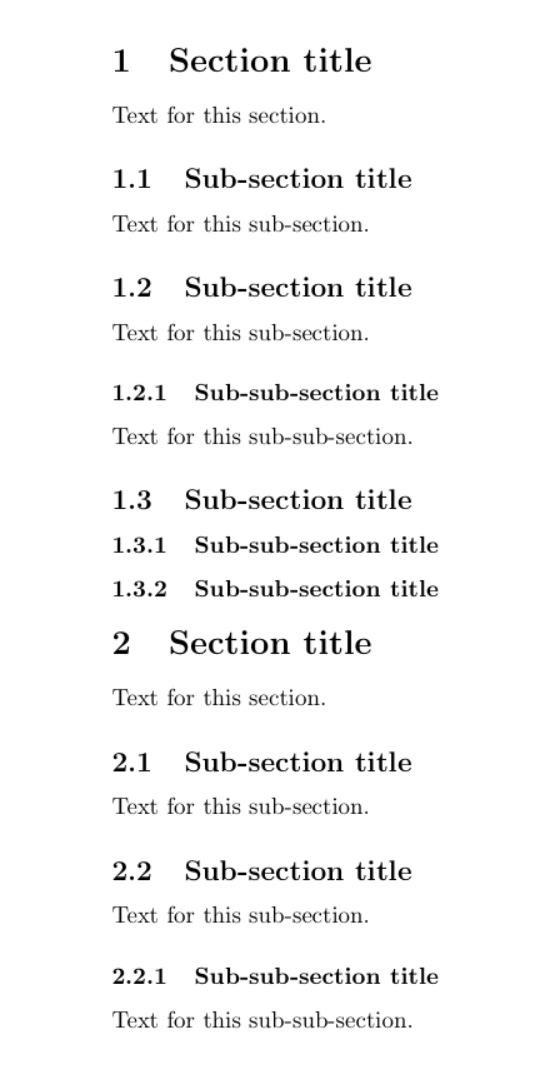
\includegraphics[width=0.3\textwidth]{figures/L05/overleafSections.png}}
    \caption{Some sectioned text generated by \LaTeX{}.}
    \label{overleafNotes.fig}
\end{figure}

Once you start sectionizing your text it is quite likely that you will want to refer to a section from some other part of the text. This is easy to do using the \verb|\label| macro to give a section a label, and \verb|\ref| macro to refer to a labelled section. For instance

\begin{minted}{latex}
\begin{document}
  \section{Introduction}
  \section{Big idea}
    \label{bigIdea.sec}
    Text for the big idea.
    \subsection{Smaller idea}
      \label{smallerIdea.sec}
      Text for the smaller idea.
  \section{Justifying ideas}
    Supporting argument for the big idea in Section \ref{bigIdea.sec}. 
    
    How the smaller idea in Section \ref{smallerIdea.sec} relates to the big idea.
\end{document}
\end{minted}

When compiled 
\begin{figure}[htbp!]
    \centering
    \fbox{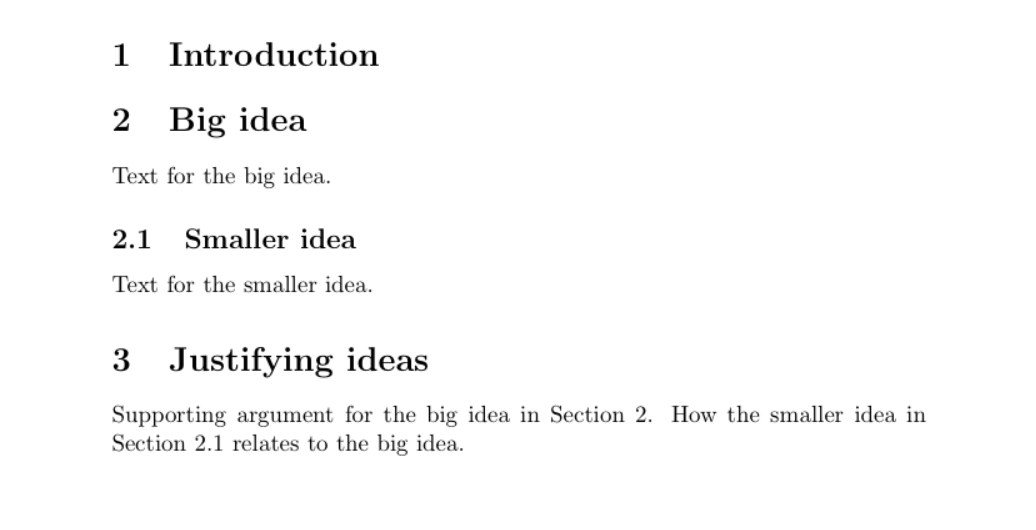
\includegraphics[width=0.8\textwidth]{figures/L05/overleafLabelRef.png}}
    \caption{References to labelled sections in \LaTeX{}.}
    \label{overleafLabelRef.fig}
\end{figure}


\section{Including math formulae}

So far you might not be too impressed by the \LaTeX{} features we have discussed  and maybe you are wondering if it is worth the loss of true WYSIWIG to get these limited features. Fear not, \LaTeX{} really shines when it comes to type setting math equations, formulae, expressions, theorems, proofs, \ldots. I cannot think of another piece of software that produces as high quality math renderings.

Typesetting math is central to \LaTeX{} and as you might imagine there are several ways to code up math expressions. In the following we give four different math environments with different features and use cases.

\subsection{Tips for finding \LaTeX{} math macro names}

\begin{tcolorbox}[colback=white]
{\bf Tip \#1}: if you need to find a \LaTeX{} math symbol macro you can try sketching the symbol on Detexify \href{http://detexify.kirelabs.org/classify.html} or this similar web app \href{http://www.martin-thoma.de/write-math/classify}{Classify}.\\

{\bf Tip \#2}: if you want to reproduce a piece of handwritten math or math from a paper you can try: Snip by \href{https://mathpix.com/}{MathPix}. There is even an Android phone app ! \\

{\bf Tip \#3}: there is a neat short guide to common \LaTeX{} constructions and symbols \href{ftp://ftp.ams.org/pub/tex/doc/amsmath/short-math-guide.pdf}{here}. \\

{\bf Tip \#4}: you can try finding the symbol by searching in this \href{http://milde.users.sourceforge.net/LUCR/Math/unimathsymbols.pdf}{document}. Note it assumes that you have loaded several packages. \\

{\bf Tip \#5}: search with your favorite search engine, for example search: \texttt{latex smiley macro}.
\end{tcolorbox}

\subsection{Inlined text environment using dollar symbols}
\begin{minted}{latex}
You can inline short a math formula into regular text with the dollar signs as follows $f(x)=\sin(x)$
\end{minted}
which becomes

\begin{tcolorbox}
You can inline short a math formula into regular text with the dollar signs as follows $f(x)=\sin(x)$.
\end{tcolorbox}

{\bf Note}: we used the \verb|\sin| macro so that \LaTeX{} knows to render this in an appropriate font and not as three separate variables $s$, $i$, and $n$. You can see the difference by trying this with and without the backslash.

\subsection{Math environment using square bracket macros}

\begin{minted}{latex}
You can create a new math environment to interleave a math equation between some text with the square
bracket macros as follows 
\[
f(x)=\sin(x).
\]
Notice how there is a period after the equation, i.e. we treat the math expression as though it
is a sentence and it should be properly punctuated.
\end{minted}
which becomes

\begin{tcolorbox}
You can create a new math environment to interleave a math equation between some text with the square bracket macros as follows 
\[
f(x)=\sin(x).
\]
Notice how there is a period after the equation, i.e. we treat the math expression as though it is a sentence and it should be properly punctuated.
\end{tcolorbox}

With this approach the math expression is more prominent in the text. 

\subsection{Math environment using the equation environment}

We can use a slightly more sophisticated math environment 
\begin{minted}{latex}
\begin{equation}
f(x)=\sin(x).
\end{equation}
\end{minted}
This has one useful difference to the square brackets in that it will add an equation number as default behavior as 
\begin{tcolorbox}
\begin{equation}
f(x)=\sin(x).
\end{equation}
\end{tcolorbox}
Notice the equation label that appears by magic to the right of the math expression. Just as with sections you can also add a label to this math section using the \verb|\label| macro and reference it by equation number using the \verb|\ref| macro.

\subsection{Math environment for multiple equations}

Quite often we need to type up a sequence of math expressions for instance in proving some inequality. We can use the \texttt{eqnarray} enviroment to do this while neatly aligning the sequence of equations as in the following example

\begin{minted}{latex}
A simple proof of the \href{https://en.wikipedia.org/wiki/Cauchy–Schwarz_inequality}{Cauchy-Schwarz inequality} that $|u\cdot v| \leq \|u\| \|v\|$  for all $u,v\in \mathbb{R}^N$ starts with a trivially true statement
\begin{eqnarray}
0 & \leq & \| \left( u \|v\|^2 - v (u\cdot v) \right) \|^2, \\
  & = & (u \|v\|^2 - v (u\cdot v))\cdot(u \|v\|^2 - v (u\cdot v)),\\
  & =  & \|u\|^2\|v\|^4 - 2(u\cdot v)^2\|v\|^2 + \|v\|^2 (u\cdot v)^2,\\
  & = &  \|u\|^2\|v\|^4 - (u\cdot v)^2\|v\|^2,
\end{eqnarray}
and if $\|v\|>0$ then we can divide both sides of the inequality by $\|v\|^2$ and then take the square
root of both sides of the inequality. This implies
\[
\|u\|\|v\| > |u\cdot v|
\]
as claimed.
\end{minted}
becomes
\begin{tcolorbox}
A simple proof of the \href{https://en.wikipedia.org/wiki/Cauchy–Schwarz_inequality}{Cauchy-Schwarz inequality} 
that $|u\cdot v| \leq \|u\| \|v\|$  for all $u,v\in \mathbb{R}^N$ 
starts with a trivially true statement
\begin{eqnarray}
0 & \leq & \| \left( u \|v\|^2 - v (u\cdot v) \right) \|^2, \\
  & = & (u \|v\|^2 - v (u\cdot v))\cdot(u \|v\|^2 - v (u\cdot v)),\\
  & =  & \|u\|^2\|v\|^4 - 2(u\cdot v)^2\|v\|^2 + \|v\|^2 (u\cdot v)^2,\\
  & = &  \|u\|^2\|v\|^4 - (u\cdot v)^2\|v\|^2,
\end{eqnarray}
and if $\|v\|>0$ then we can divide both sides of the inequality by $\|v\|^2$ and then take the square 
root of both sides of the inequality. This implies
\[
\|u\|\|v\| > |u\cdot v|
\]
as claimed.
\end{tcolorbox}
{\bf Note \#1}: how we use each of  three math environments as required to inline a short expression, separate a key result, or align multiple expressions. 

{\bf Note \#2}: \LaTeX{} has added an equation number to each of the lines of the \verb|eqnarray| environment. You can turn off the line numbering by instead using the \verb|eqnarray*| environment.

{\bf Note \#3}: \LaTeX{} has neatly aligned all of the equations in the \verb|eqnarray| environment at the symbol between the ampersands.

\section{Including an image from file}

You will have noticed that there are figures throughout this text. Unfortunately I suspect that you have also noticed that sometimes the figures are placed in what seems like a haphazard way, occasionally quite distant from a seemingly natural placement. I encourage you to read Leslie Lamport's writings on whether an author should be responsible for dictating the visual layout of a document or the logical document layout \cite{lamport1988document}. As the creator of \LaTeX{} his viewpoint is that the author should pay attention mostly to the flow of thoughts in a document and let the typesetting software make the majority of decisions in visual presentation of the material. This is most evident in the way \LaTeX{} chooses to insert figures in text. The priority for \LaTeX{} is to prioritize readability with the location of figures and their proximity to where they might be cited being a very much subsidiary concern.

\begin{figure}[htbp!]
    \begin{center}
      \includegraphics[width=0.5\textwidth]{figures/L05/overleafExampleImage.jpg}
    \end{center}
    \caption{Caption for example figure}
    \label{exampleFigure.fig}
\end{figure}


Figures are introduced into the text using macros of course. Here is an example of \LaTeX{} macro that adds a figure using the \texttt{includegraphics} macro embedded inside a \texttt{figure} environment to produce Figure \ref{exampleFigure.fig}.

\begin{minted}{latex}
\begin{figure}[htbp!]
    \begin{center}
      \includegraphics[width=0.5\textwidth]{figures/L05/overleafExampleImage.jpg}
    \end{center}
    \caption{Caption for example figure}
    \label{exampleFigure.fig}
\end{figure}
\end{minted}

{\bf Note \#1}: the \texttt{figure} environment has an optional argument given in the square brackets. This string [htbp!] specifies the preference for this figure. In this case h=here, t=top, b=bottom, p=page, and the exclamation mark indicates this is a high priority.

{\bf Note \#2}: we choose to center the image about the vertical by using the \texttt{center} environment.

{\bf Note \#3}: we specify the figure and path when using the \texttt{includegraphics} macro. The optional argument in the square brackets indicates that the image should be one half of the text width for the document.

{\bf Note \#4}: the caption macro includes the text to be added for the caption as an argument. If you insert the caption above the \texttt{includegraphics} then the caption will appear above the image.

{\bf Note \#5}: the caption will include the text ``Figure'' and a figure number. Adding a label with the \texttt{label} macro allows us to reference this figure by number using the \texttt{ref} macro. In this case we would reference the figure with \verb|\ref{exampleFigure.fig}|.

{\bf Note \#6}: in general for figures with graphs and charts it is advisable to use a vector graphics format file where possible. MATLAB and other plotting tools can often create vector graphics formatted files (for instance pdf) that can be scaled in size without loss of quality.

{\bf Note \#6}: the \texttt{includegraphics} command is part of the \texttt{graphicx} package. You should make sure you include this package by adding the following to your preamble.

\begin{minted}{latex}
\usepackage{graphicx}
\end{minted}

\section{Plotting a figure directly in \LaTeX{}}

Sometimes if you have a fairly simple dataset it may be possible to directly plot a chart/graph directly using macros in \LaTeX{}. This will let you build self contained \LaTeX{} projects where if the data changes you can just enter new values into your .tex file and recompile. 

The \texttt{tikz},\texttt{pgf} packages are a reasonable place to start when you just need to generate simple charts directly via \LaTeX{} macros. There is even a \href{https://en.wikipedia.org/wiki/PGF/TikZ}{wiki} entry for using these packages. In the following we give an example of a simple chart generated entirely within \LaTeX{} document macros.

\subsection{Plotting a chart with \texttt{tikz},\texttt{pgf}}
We first include the following in the document preamble
\begin{minted}{latex}
\usepackage{pgf,tikz}
\usepackage{pgfplots}
\end{minted}

The following \LaTeX{} example uses the \texttt{tikzpicture} environment within a \texttt{figure} environment to create the plot shown in Figure \ref{exampleGraph.fig}.

\begin{minted}{latex}
\begin{figure}[htbp]
\centering
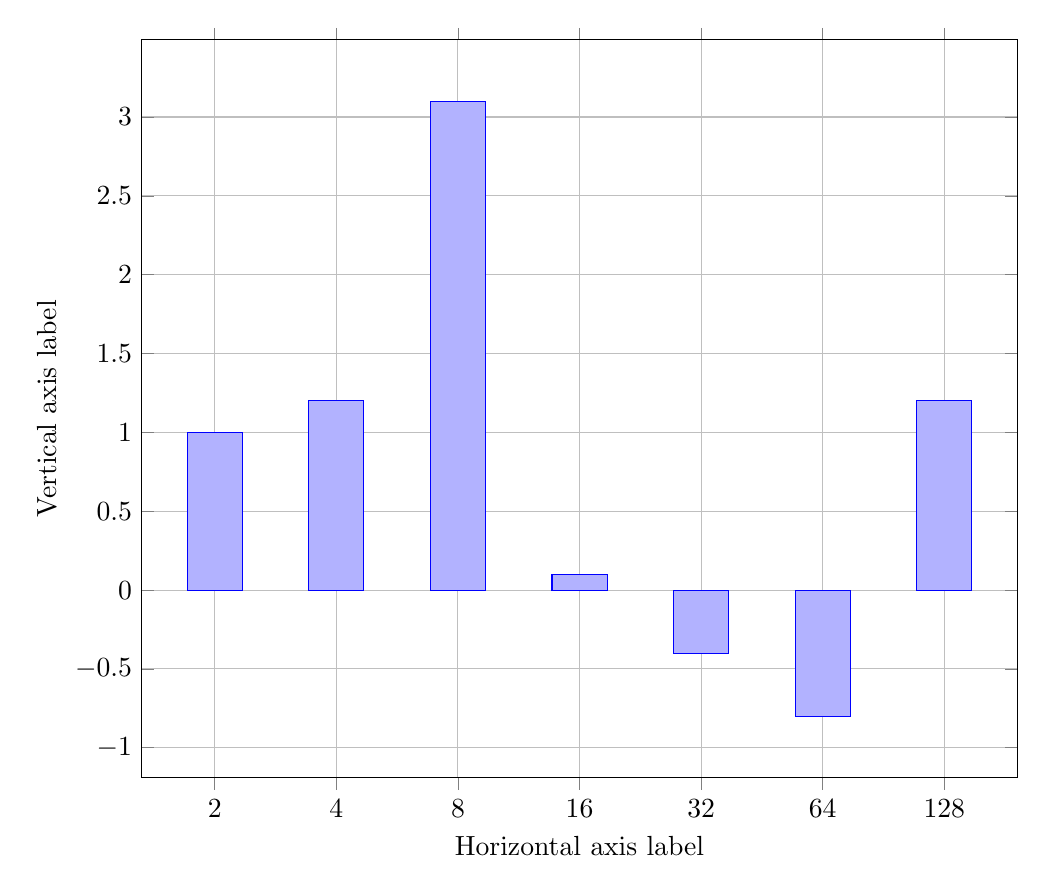
\begin{tikzpicture}
\begin{axis}[
    width=5in, % axis width
    ybar,   % specify use bar plot
    enlargelimits=0.1, % padding around limits
    xlabel={Horizontal axis label}, % x axis label
    ylabel={Vertical axis label}, % y axis label
    symbolic x coords={2,4,8,16,32,64,128},
    xtick=data, % specify type of ticks on x axis
    grid=major, % enable major grid 
    bar width=0.7cm, % width of bars
    ]
%% These are coordinates of points to plot
\addplot coordinates {(2, 1) (4, 1.2) (8, 3.1) (16, .1) (32,-.4) (64,-.8) (128,1.2)};
\label{exampleGraph.fig}
\end{axis}
\end{tikzpicture}
    \caption{Example graph plotted from within \LaTeX{} using the \texttt{tikzpicture} package. }
    \label{exampleGraph.fig}
\end{figure}
\end{minted}

\begin{figure}[htbp]
\centering
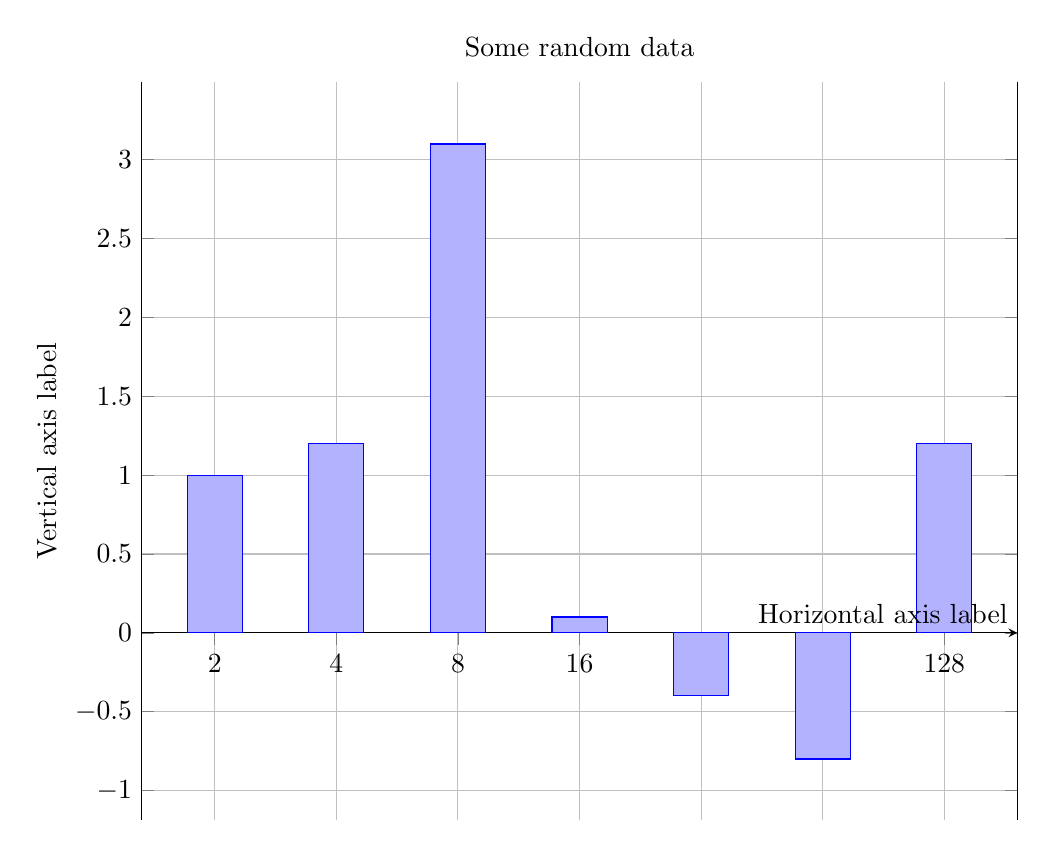
\begin{tikzpicture}
\begin{axis}[
    width=5in,
    axis x line=middle,
    ybar,%=8pt, % configures ‘bar shift’
    enlargelimits=0.1,
    xlabel={Horizontal axis label},
    ylabel={Vertical axis label},
    symbolic x coords={2,4,8,16,32,64,128},
    xtick=data,
    grid=major,
    bar width=0.7cm,
    title={Some random data},
    ]
%% These are coordinates of points to plot
\addplot coordinates {(2, 1) (4, 1.2) (8, 3.1) (16, .1) (32,-.4) (64,-.8) (128,1.2)};
\label{exampleGraph.fig}
\end{axis}
\end{tikzpicture}
    \caption{Example graph plotted from within \LaTeX{} using the \texttt{tikzpicture} package. }
    \label{exampleGraph.fig}
\end{figure}

\subsection{Making a scatter plot directly in \LaTeX{}}
LaTeX{} can also use data from another file.
Say you have the following data saved in a file called \texttt{scatterdata.txt}
\begin{tsession}{mycodebg}
\begin{verbatim}
x  y          cluster
0  0.0        1
1  162.25     1
2  256.5      1
3  288.75     2
4  265.0      2
5  191.25     2
6  73.5       3
7  -82.25     3
8  -270.0     3
9  -483.75    4
10 -717.5     4
11 -965.25    4
12 -1221.0    5
13 -1478.75   5
14 -1732.5    5
15 -1976.25   6
16 -2204.0    6
17 -2409.75   6
18 -2587.5    7
19 -2731.25   7
20 -2835.0    7
21 -2892.75   8
22 -2898.5    8
23 -2846.25   8
24 -2730.0    9
25 -2543.75   9
26 -2281.5    9
27 -1937.25  10
28 -1505.0   10
29 -978.75   10
30 -352.5    11
31 379.75    11
32 1224.0    11
33 2186.25   12
34 3272.5    12
35 4488.75   12
\end{verbatim}
\end{tsession}
 And say you want to plot the data with different colors for points in each cluster.
 A tikzpicture can read the data directly from the file,
 as shown in the next code.
 The command also specifies the colors for the markers of each cluster.
\begin{minted}{latex}
\documentclass{article}
\begin{tikzpicture}[scale=1.5] % Scale can increase size of axis along with text and markers
\begin{axis}[
height=3in, % specify height and width of axis
width=4in,
scatter/classes={
    1={mark=*,fill=magenta},
    2={mark=*,fill=red},
    3={mark=*,fill=orange},
    4={mark=*,fill=yellow},
    5={mark=*,fill=green},
    6={mark=*,fill=cyan},
    7={mark=*,fill=teal},
    8={mark=*,fill=blue},
    9={mark=*,fill=violet},
    10={mark=*,fill=black},
    11={mark=*,fill=gray},
    12={mark=*,fill=white}
},
xlabel=x-coordinate, % Add labels to axes
ylabel=y-coordinate,
title=Appropriate title % Add title
]
\addplot[scatter,only marks,scatter src=explicit symbolic]
file[skip first]{scatterdata.txt}; % Tell LaTex where to find data and skip the first line (a header)
\end{axis}
\end{tikzpicture}
\end{minted}
Figure~\ref{fig:pic_from_file} shows the resulting picture.

\begin{figure}[htbp!]
    \centering
    \begin{tikzpicture}[scale=1.5] % Scale can increase size of axis along with text and markers
\begin{axis}[
height=3in, % specify height and width of axis
width=4in,
scatter/classes={
    1={mark=*,fill=magenta},
    2={mark=*,fill=red},
    3={mark=*,fill=orange},
    4={mark=*,fill=yellow},
    5={mark=*,fill=green},
    6={mark=*,fill=cyan},
    7={mark=*,fill=teal},
    8={mark=*,fill=blue},
    9={mark=*,fill=violet},
    10={mark=*,fill=black},
    11={mark=*,fill=gray},
    12={mark=*,fill=white}
},
xlabel=x-coordinate, % Add labels to axes
ylabel=y-coordinate,
title=Appropriate title % Add title
]
\addplot[scatter,only marks,scatter src=explicit symbolic]
file[skip first]{figures/L05/scatterdata.txt}; % Tell LaTex where to find data and skip the first line (a header)
\end{axis}
\end{tikzpicture}
    \caption{Graph using data from the file \texttt{scatterdata.txt}.}
    \label{fig:pic_from_file}
\end{figure}

For a collection of example data representations see \href{http://pgfplots.sourceforge.net/gallery.html}{here}.

\section{Building a bibliography}

A simple rule of thumb when writing is that if your work relies on an idea from a paper, a theorem proved in a thesis, a conjecture from a lecture, a data set, a measurement standard, a concept from a book, an algorithm from the literature, mathematical software, a software library, a design from a web page, an idea from a colleague then it is your responsibility to cite the source. The VT library has some resources on when to cite \href{https://guides.lib.vt.edu/citationmanagers}{here} and some tools to manage citations.

In this section we will discuss how to cite prior work. The main tool we will use is the \LaTeX{}  \texttt{bibilography} environment. The idea is simple: create a \texttt{[BIBLIOGRAPHY].bib} file that includes a formatted record for every source that you wish to cite. Once upon a time research groups would build a \texttt{.bib} file and guard it jealously as it took significant time to track down and transcribe bibliography entries in the appropriate record format. 

These days it is much easier to create a bibliography file. The first step is to create a \texttt{[BIBLIOGRAPHY].bib} file attached to your working project on \href{https://overleaf.com}{overleaf.com}. I will assume you are familiar with using \href{https://scholar.google.com}{scholar.google.com} to find academic books and journal articles. If you are not then now is the time to pick up that habit. 

You will be using \href{https://scholar.google.com}{scholar.google.com}  to collect bibliography records for every article that you read. To set up go to \href{https://scholar.google.com}{scholar.google.com}  and navigate to the settings panel and select ``Show links to import into bibtex''.

\boximage{figures/L05/scholarGoogleSettings.png}{Settings page for \href{https://scholar.google.com}{scholar.google.com}. Make sure to click ``Show links to import into bibtex''.}

Now go back to the main \href{https://scholar.google.com}{scholar.google.com} page and use the search dialog box to find references to some subject or authors as shown in Figure \ref{scholarGoogleSearch.fig}.

\boximagelabel{figures/L05/scholarGoogleSearch.png}{Searching for a two author work on \href{https://scholar.google.com}{scholar.google.com}}{scholarGoogleSearch.fig}

The scholar.google website maintains a huge searchable database of journal articles, books, conference papers, preprints, and even patents. It is the most comprehensive database of academic works that I am aware of. Even more important than the size of the database is the way that articles are cross referenced and also that many academic authors maintain curated lists of their work. The above search gives the  somewhat familiar looking search results shown in Figure \ref{scholarGoogleSearchResults.fig}.

\boximagelabel{figures/L05/scholarGoogleSearchResults.png}{Search results for query on\href{https://scholar.google.com}{scholar.google.com}. }{scholarGoogleSearchResults.fig}

The key things to observe:

{\bf Note \#1}: The titles of each search result are clickable and will take you to a journal, preprint server, or publisher website. 

{\bf Note \#2}: Many authors are clickable and the links will take you to their curated publications collection.

{\bf Note \#3}: Many articles are behind pay walls. Fortunately VT has extensive journal and publisher subscriptions.

{\bf Note \#4}: If VT does not have access rights for an article you might be able to find a preprint version by clicking on "All \#\# versions". 

{\bf Note \#5}: You can collect a bibliography entry by clicking on the quotation marks for an article. See Figure \ref{scholarGoogleSearchResultsCite.fig} for an example. Go ahead and click on the BibTeX button. 

\boximagelabel{figures/L05/scholarGoogleSearchResultsCite.png}{Bibliograrphy entry for a search results  on\href{https://scholar.google.com}{scholar.google.com}. }{scholarGoogleSearchResultsCite.fig}

You will be presented with a text bibliography entry that \LaTeX{} can use. Copy and paste the entry from the browser into your \href{https://overleaf.com}{overleaf.com} [BIBLIOGRAPHY].bib file. My exampple is as follows

\begin{minted}{latex}
@book{hesthaven2007nodal,
  title={Nodal discontinuous Galerkin methods: algorithms, analysis, and applications},
  author={Hesthaven, Jan S and Warburton, Tim},
  year={2007},
  publisher={Springer Science \& Business Media}
}
\end{minted}

The first string in the bibliography (here \texttt{hesthaven2007nodal} is a label you can use to cite the work. To cite this work in a \LaTeX{} document you can write something like the following.

\begin{minted}{latex}
This method is based on the nodal discontinuous Galerkin discretization described in by 
Hesthaven and Warburton \cite{hesthaven2007nodal}.
\end{minted}

By citing the book here \cite{hesthaven2007nodal} \LaTeX{} will automatically add a reference entry to the bibliography that you can find at the end of the chapter. 

In your \LaTeX{} document you should add the following text at the end of the main .tex file before the \texttt{end\{document\}} macro.

\section{Creating new \LaTeX{} commands}

So far we have used macros that are built into \LaTeX{} and supplied by add-on packages. It is important to understand that \LaTeX{} is an extensible macro language, i.e. we can define our own macros for new macro commands that we wish to perform tasks that we find ourselves doing multiple times. See \href{https://en.wikibooks.org/wiki/LaTeX/Macros}{wiki} for a more in depth discussion.

As an example imagine that we frequently want to use {\color{red}{red}} highlighting in a piece of text. Assuming you have already setup color names by adding this to your preamble  

\begin{minted}{latex}
\usepackage[usenames,dvipsnames]{xcolor}
\end{minted}

You can wrap the a piece of text with this macro and syntax to make it red

\begin{minted}{latex}
{\color{red}{[YOUR TEXT]}}
\end{minted}

Doing this everywhere you want to highlight text in red is a bit of a pain. Worse still, what happens if you realize some 8\% of the population are color blind to red and that red text generates negative reactions in the other 92\% ? You decide to use blue and have to go through fixing the highlight color everywhere. What a pain !

Thus it makes a lot of sense to define a new macro text callout coloring macro in your preamble that you can use everywhere. If you change your mind about how you want the callout to highlight text you can adjust what the macro does in the preamble and the changes will propagate throughout the document the next time you compile the document.

To define a macro called \texttt{mycall} that takes argument you can add this to your preamble.

\begin{minted}{latex}
\newcommand{\mycall}[1]{\textcolor{red}{#1}}
\end{minted}

Then when you want to use this macro in the body of the \LaTeX{} document you can do the following.

\begin{minted}{latex}
\mycall{This is some text that we want to highlight}. And this is text we do not want to highlight.
\end{minted}

If you want to create a macro with two or more arguments then you increase the first optional argument to the \texttt{newcommand} macro as in the following macro where we actually pass the color in as an argument.

\begin{minted}{latex}
\newcommand{\mycall}[2]{\textcolor{#1}{#2}}
\end{minted}

We can invoke this macro as in the following example.

\begin{minted}{latex}
\mycall{red}{This is some text that we want to highlight}. And this is text we do not want to highlight.
\end{minted}

In fact we use that macro in this line of the lecture notes to \mycall{blue}{highlight some random text}. 

But hold on you say ! We have just created an alias for the \texttt{textcolor} macro. Good point. So let's up the ante and insist that the callout makes the text bold as well as setting the color with.

\begin{minted}{latex}
\newcommand{\mycall}[2]{{\bf \color{#1}{#2}}}
\end{minted}

Making this change to the callout macro will now bold as well as color your highlighted text throughout the document on the next compile.

{\bf Note}: \LaTeX{} will complain if you try to define a new macro that has the same name as an existing macro. I would suggest choosing a different name for your new macro. If you are insistent on using the name for your new macro then you can use the \texttt{renewcommand} instead of the \texttt{newcommand} in your declaration.
%%\section{Formatted pseudo-code}

\section{Formatted source code listings}

A quick guide to nicely formatting your source code listings when including them in a \LaTeX{} document.

Let's consider a simple piece of C code that for some reason you would like to include in a document, perhaps as part of a project report. You could use the \verb|verbatim| environment but the result will be rather basic

\begin{verbatim}
#include <stdio.h>

int main(int argc, char **argv){

   printf("hello world\n");

  return 0;
}
\end{verbatim}
The code is not really distinct from the surrounding text. There is no color highlighting of keywords. There are no line numbering, no caption, ...

To create more distinctive source code listings I  recommend using the \href{https://www.overleaf.com/learn/latex/Code_Highlighting_with_minted}{minted} package for \LaTeX{}. It extends the verbatim environment to include formatting options like color coded syntax, line numbers, and framed listings. You could also use the \href{https://www.overleaf.com/learn/latex/Code_listing}{lstlistings} package which has similar features.

The first thing to do is to include the minted package in your package by adding this to your preamble 
\begin{minted}{latex}
\usepackage{minted}
\end{minted}

I usually add default formatting options for the minted display of C and \LaTeX{}. I addd the following to my preamble after the minted \texttt{usepackage} macro to add a line around the listing, set the background to a gray, specify small font, and enable line numbers.

\begin{minted}{latex}
\definecolor{mygray}{rgb}{0.95,0.95,0.95}

\setminted[c]{autogobble=true, frame=lines, framesep=4mm, baselinestretch=1.2, 
bgcolor=mygray, fontsize=\footnotesize,linenos=true}

\setminted[latex]{autogobble=true, frame=lines, framesep=4mm, baselinestretch=1.2, 
bgcolor=mygray, fontsize=\footnotesize,linenos=true}
\end{minted}

With these options in place we can use the following \LaTeX{} to render the above example code

\begin{verbatim}
\begin{minted}{c}
#include <stdio.h>

int main(int argc, char **argv){

   printf("hello world\n");

  return 0;
}
\end{minted}
\end{verbatim}

which produces

\begin{minted}{c}
#include <stdio.h>

int main(int argc, char **argv){

   printf("hello world\n");

  return 0;
}
\end{minted}
Notice how the C types are highlighted in maroon, the main function in blue, the compiler directives in yellow (?), the string in brown (?), and the return keyword is shown in green. If you do not like the color scheme this can of course be customized.

If you include source code in your homework report you should use the minted or lstlistings package in \LaTeX{}. Just by adding the preamble code above and the \texttt{minted} commands in the body of your document you get nicely formatted source code with almost zero effort.

\printbibliography[heading=subbibliography]